\documentclass[tikz,border=10pt]{standalone}
\usepackage[T1]{fontenc}
\usepackage{mathpazo}
\usetikzlibrary{arrows.meta, positioning, calc, fit}

\definecolor{stblue}{HTML}{7B97AD}
\definecolor{rwgold}{HTML}{B8995E}
\definecolor{sage}{HTML}{7A9A7E}
\definecolor{dkbrown}{HTML}{3D3530}
\definecolor{wmgray}{HTML}{7B7067}
\definecolor{cream}{HTML}{F9F6F0}
\definecolor{border}{HTML}{D4C9B8}

\begin{document}
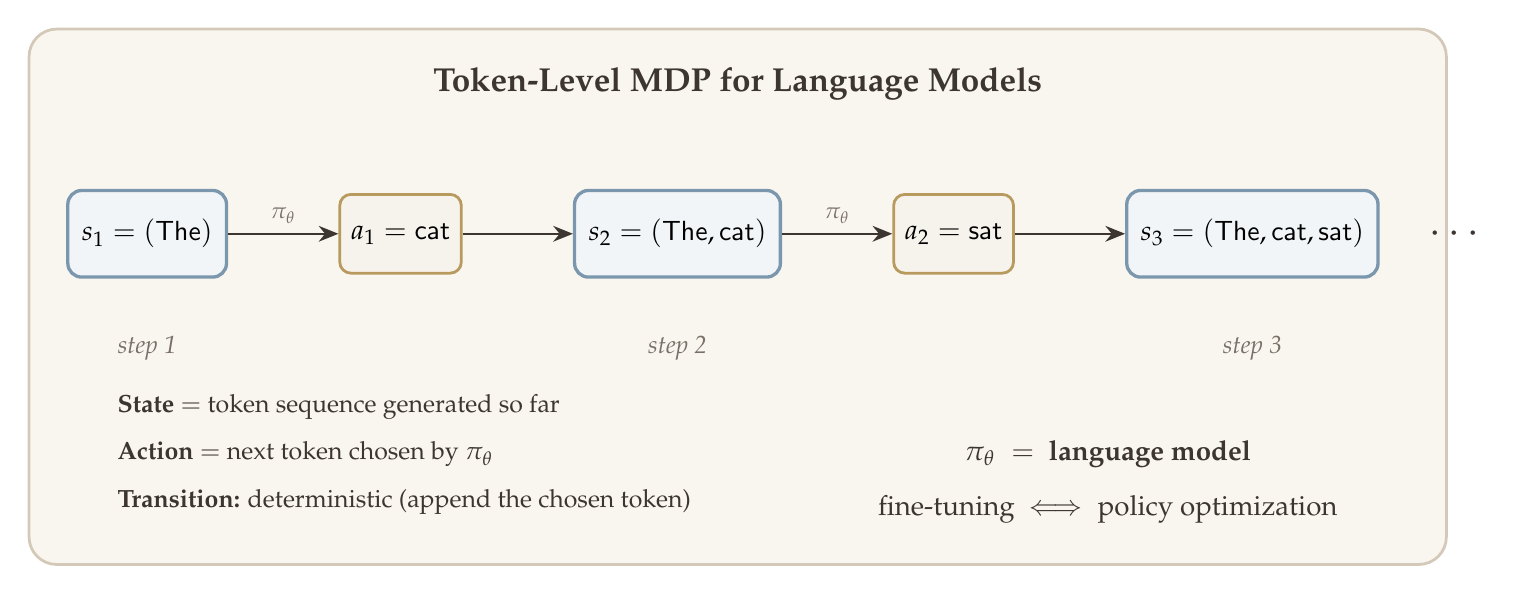
\begin{tikzpicture}[
  >={Stealth[length=2.5mm, width=2mm]},
  arr/.style={draw=dkbrown, line width=0.9pt, ->},
  state/.style={rectangle, rounded corners=5pt, draw=stblue, line width=1.2pt,
    fill=stblue!10, minimum height=11mm, inner sep=5pt, font=\normalsize},
  action/.style={rectangle, rounded corners=4pt, draw=rwgold, line width=1pt,
    fill=rwgold!12, minimum height=10mm, inner sep=4pt, font=\normalsize},
  note/.style={font=\small\itshape, text=wmgray},
]

% Background
\fill[cream, rounded corners=10pt] (-1.5,-4.2) rectangle (16.5,2.6);
\draw[border, rounded corners=10pt, line width=1pt] (-1.5,-4.2) rectangle (16.5,2.6);

% Title
\node[font=\large\bfseries, text=dkbrown] at (7.5,1.9) {Token-Level MDP for Language Models};

% === Row of states and actions ===

% Step 1: state
\node[state] (s1) at (0,0) {$s_1 = (\textsf{The})$};

% Step 1: action
\node[action, right=14mm of s1] (a1) {$a_1 = \textsf{cat}$};
\draw[arr] (s1) -- node[above, font=\footnotesize, text=wmgray] {$\pi_\theta$} (a1);

% Step 2: state
\node[state, right=14mm of a1] (s2) {$s_2 = (\textsf{The}, \textsf{cat})$};
\draw[arr] (a1) -- (s2);

% Step 2: action
\node[action, right=14mm of s2] (a2) {$a_2 = \textsf{sat}$};
\draw[arr] (s2) -- node[above, font=\footnotesize, text=wmgray] {$\pi_\theta$} (a2);

% Step 3: state
\node[state, right=14mm of a2] (s3) {$s_3 = (\textsf{The}, \textsf{cat}, \textsf{sat})$};
\draw[arr] (a2) -- (s3);

% Continuation
\node[font=\Large, text=dkbrown, right=5mm of s3] {$\cdots$};

% Step labels
\node[note, below=6mm of s1] {step 1};
\node[note, below=6mm of s2] {step 2};
\node[note, below=6mm of s3] {step 3};

% === Annotation table: three columns, cleanly separated ===
\node[font=\small, text=dkbrown, anchor=west] at (-0.5,-2.2)
  {\textbf{State} $=$ token sequence generated so far};
\node[font=\small, text=dkbrown, anchor=west] at (-0.5,-2.8)
  {\textbf{Action} $=$ next token chosen by $\pi_\theta$};
\node[font=\small, text=dkbrown, anchor=west] at (-0.5,-3.4)
  {\textbf{Transition:} deterministic (append the chosen token)};

% Punchline
\node[font=\normalsize\bfseries, text=dkbrown] at (12.2,-2.8)
  {$\pi_\theta \;=\;$ language model};
\node[font=\normalsize, text=dkbrown] at (12.2,-3.5)
  {fine-tuning $\;\Longleftrightarrow\;$ policy optimization};

\end{tikzpicture}
\end{document}
